%%%%%%%%%%%%%%%%%%%%%%%%%%%%%%%%%%%%%%%%%
% University Assignment Title Page 
% LaTeX Template
% Version 2.1 (18/10/18)
% Modified by
% Erdem TUNA &
% Halil TEMURTAŞ &
% Enes TAŞTAN
%%%%%%%%%%%%%%%%%%%%%%%%%%%%%%%%%%%%%%%%%
%
%----------------------------------------------------------------------------------------
%	PACKAGES AND OTHER DOCUMENT CONFIGURATIONS
%----------------------------------------------------------------------------------------
\documentclass[a4paper,12pt]{article}
%-----packages------
\usepackage[a4paper, total={6.2in, 9in}]{geometry}
\usepackage[english]{babel}
\usepackage[utf8x]{inputenc}
\usepackage{amsmath}
\usepackage{graphicx}
\usepackage[colorinlistoftodos]{todonotes}
\usepackage{gensymb} % this could be problem
\usepackage{float}
\usepackage{fancyref}
\usepackage{subcaption}
\usepackage[titletoc]{appendix} %appendix package
\usepackage{xcolor}
\usepackage{listings}
\usepackage{xspace}
\usepackage{amssymb}
\usepackage{nicefrac}
\usepackage{gensymb}
\usepackage{fancyhdr}
\usepackage{lipsum}  % for dummy text \lipsum[1-4]
\usepackage[final]{pdfpages}  % pdf include
%\usepackage{array} %allows more options in tables
\usepackage{pgfplots,pgf,tikz} %coding plots in latex
%\usepackage{capt-of} % allows caption outside the figure environment
\usepackage[export]{adjustbox} %more options for adjusting the images
%\usepackage{multicol,multirow,slashbox} % allows tables like table1
%\usepackage[hyperfootnotes=false]{hyperref} % clickable references
%\usepackage{epstopdf} % useful when matlab is involved
%\usepackage{placeins} % prevents the text after figure to go above figure with \FloatBarrier 
%\usepackage{listingsutf8,mcode} %import .m or any other code file mcode is for matlab highlighting
\usepackage{setspace}
%-----end of packages




%-----specifications-----
\definecolor{mGreen}{rgb}{0,0.6,0} % for python
\definecolor{mGray}{rgb}{0.5,0.5,0.5}
\definecolor{mPurple}{rgb}{0.58,0,0.82}
\definecolor{mygreen}{RGB}{28,172,0} % color values Red, Green, Blue for matlab
\definecolor{mylilas}{RGB}{170,55,241}

\setcounter{secnumdepth}{5} % how many sectioning levels to assign numbers to
\setcounter{tocdepth}{5}    % how many sectioning levels to show in ToC

\lstdefinestyle{CStyle}{
	commentstyle=\color{mGreen},
	keywordstyle=\color{magenta},
	numberstyle=\tiny\color{mGray},
	stringstyle=\color{mPurple},
	basicstyle=\footnotesize,
	breakatwhitespace=false,         
	breaklines=true,
	frame=single,
	rulecolor=\color{black!40},                 
	captionpos=b,                    
	keepspaces=true,                 
	numbers=left,                    
	numbersep=5pt,                  
	showspaces=false,                
	showstringspaces=false,
	showtabs=false,                  
	tabsize=2,
	language=C
}

\lstset{language=Matlab,%
	%basicstyle=\color{red},
	breaklines=true,%
	frame=single,
	rulecolor=\color{black!40},
	morekeywords={matlab2tikz},
	keywordstyle=\color{blue},%
	morekeywords=[2]{1}, keywordstyle=[2]{\color{black}},
	identifierstyle=\color{black},%
	stringstyle=\color{mylilas},
	commentstyle=\color{mygreen},%
	showstringspaces=false,%without this there will be a symbol in the places where there is a space
	numbers=left,%
	numberstyle={\tiny \color{black}},% size of the numbers
	numbersep=9pt, % this defines how far the numbers are from the text
	emph=[1]{for,end,break},emphstyle=[1]\color{red}, %some words to emphasise
	%emph=[2]{word1,word2}, emphstyle=[2]{style},    
}


\tikzset{
	desicion/.style={
		diamond,
		draw,
		text width=4em,
		text badly centered,
		inner sep=0pt
	},
	block/.style={
		rectangle,
		draw,
		text width=10em,
		text centered,
		rounded corners
	},
	cloud/.style={
		draw,
		ellipse,
		minimum height=2em
	},
	descr/.style={
		fill=white,
		inner sep=2.5pt
	},
	connector/.style={
		-latex,
		font=\scriptsize
	},
	rectangle connector/.style={
		connector,
		to path={(\tikztostart) -- ++(#1,0pt) \tikztonodes |- (\tikztotarget) },
		pos=0.5
	},
	rectangle connector/.default=-2cm,
	straight connector/.style={
		connector,
		to path=--(\tikztotarget) \tikztonodes
	}
}

\tikzset{
	desicion/.style={
		diamond,
		draw,
		text width=4em,
		text badly centered,
		inner sep=0pt
	},
	block/.style={
		rectangle,
		draw,
		text width=10em,
		text centered,
		rounded corners
	},
	cloud/.style={
		draw,
		ellipse,
		minimum height=2em
	},
	descr/.style={
		fill=white,
		inner sep=2.5pt
	},
	connector/.style={
		-latex,
		font=\scriptsize
	},
	rectangle connector/.style={
		connector,
		to path={(\tikztostart) -- ++(#1,0pt) \tikztonodes |- (\tikztotarget) },
		pos=0.5
	},
	rectangle connector/.default=-2cm,
	straight connector/.style={
		connector,
		to path=--(\tikztotarget) \tikztonodes
	}
}
%-----end of specifications-----


%----commands----
\newcommand\nd{\textsuperscript{nd}\xspace}
\newcommand\rd{\textsuperscript{rd}\xspace}
\newcommand\nth{\textsuperscript{th}\xspace} %\th is taken already
\newcommand{\specialcell}[2][c]{ \begin{tabular}[#1]{@{}c@{}}#2\end{tabular}} % for too long table lines

\newcommand{\blankpage}{
	\- \\[9cm]	
	{ \centering \textit{This page intentionally left blank.} \par }
	\- \\[9cm]
}% For Blank Page

\makeatletter
\renewcommand\paragraph{\@startsection{paragraph}{4}{\z@}%
	{-2.5ex\@plus -1ex \@minus -.25ex}%
	{1.25ex \@plus .25ex}%
	{\normalfont\normalsize\bfseries}}
\makeatother
%-----end of commands-----
\onehalfspacing
\begin{document}

\begin{titlepage}

\newcommand{\HRule}{\rule{\linewidth}{0.5mm}} % Defines a new command for the horizontal lines, change thickness here
\centering 


\includegraphics[width=\textwidth,height=\textheight,keepaspectratio]{../../Documents/logos/logo3-with-stroke}\\[0.5cm]

\textsc{\LARGE Middle East Technical University}\\[0.5cm] % Name of your university/college
\textsc{\Large Department of \\Electrical and Electronics Engineering }\\[0.5cm] % Major heading such as course name
\textsc{\large EE493 ENGINEERING DESIGN I}\\[0.5cm] % Minor heading such as course title


\HRule \\[0cm]
{ \huge \bfseries  Car Chasing Robot\\[0.1cm] \LARGE \bfseries Proposal Report}\\[0cm] % Title of your document
\HRule \\[1cm]

\begin{minipage}[l]{0.6\textwidth}
\raggedright
		\large{\textbf{Supervisor:}}	Assoc. Prof. Emre Özkan \\
		\hspace{3.05cm}\color{red} ADDDRESSS

\end{minipage}
\begin{minipage}[r]{0.35\textwidth}
\raggedright
		\textbf{Project Start:} 4/10/2018\\
		\textbf{Project End:} \ \  26/5/2019\\
		\textbf{Project Budget:} \$450

\end{minipage}\\[1cm]
\begin{minipage}{\textwidth}
	\begin{flushleft}
		\large{\textbf{Company Name :}}	Duayenler Ltd. Şti.\\
		\begin{table}[H]
			\begin{tabular}{l l l l}
				\hline
				\textbf{Members}&\textbf{Title}& \textbf{ID}&\textbf{Phone} \\ \hline
				Sarper Sertel & Electronics Engineer& 2094449 & 0542 515 6039  \\ 
				Enes Taştan & Hardware Design Engineer & 2068989 & 0543 683 4336  \\ 
				Erdem Tuna & Embedded Systems Engineer& 2617419 & 0535 256 3320  \\ 
				Halil Temurtaş & Control Engineer& 2094522 & 0531 632 2194  \\
				İlker Sağlık & Software Engineer& 2094423 & 0541 722 9573  \\ \hline
				
				
			\end{tabular}
		\end{table}
	\end{flushleft}
\end{minipage}\\[1cm]

\begin{flushbottom}
{\large November 9, 2018} % Date, change the \today to a set date if you want to be precise
\end{flushbottom}

\end{titlepage}

\blankpage
\tableofcontents
\newpage



	\section{notes}


\subsection{specific requirements and objectives of the project}


\subsection{approach to the solution of the problem}


\subsection{outline of the requirements for any standards that the product would need to comply with,}


\subsection{deliverables and expected outcomes of the project,}


\subsection{tentative cost-budget analysis,}


\section{Executive Summary}


\section{Introduction}

Driving is a common event that many people experience in their daily life. As time passes, human reflexes started to become insufficient for driving compared to fast pace of daily life in modern world. Together with the developments in the technology, new solutions are proposed to assist the driver such as lane tracking and emergency breaking systems. The ultimate version of such solutions are considered to be fully autonomous self-driving cars. \\

Self-driving vehicles are presented to the society as a solution that can facilitate people's life in many ways. Fast operation of the electronics system allows faster response than humans can. A fast and reliable operation of self-driving action can prevent many accidents and increase the safety of the roads in heavy traffics since the system is immune to human defects such as distraction and panic. As a result, autonomous vehicles can open doors to a safer and more conventional future.\\

DUAYENLER Ltd. Şti. is launched with the aim of innovating automation technologies. In that context, a device that can detect the road and other vehicles on them will be built. It autonomously track the lane and stay on the road while trying to as fast as possible.\\

This report includes;
\begin{itemize}
	\item organization of the company by explaining of the qualifications of the members. 
	\item Requirements for physically realizing the intended vehicle
	\item Possible solutions in system and subsystem levels by explaining their operations
	\item Timeline and cost of the project
	\item Expected deliverables from the project 
\end{itemize} 



\section{Our Team}

	DUAYENLER Ltd. Şti. (DUAYENLER) was founded in September 2018 by five electrical and electronics engineering students from Middle East Technical University. The company structure is shown in \textit{Figure~\ref{fig:company_tree}}. The team is composed of variously skilled visionary members. The leader of the team is Halil Temurtaş, a control engineer. Being the team leader, Halil manages the organization of the members as well as drawing an outline for the future calendar. He is experienced in using microcontrollers, device testing and project scheduling. He will be working on the development of the subsystems computation, motion and driving in parallel with his experiences. Sarper Sertel, electronics engineer, has a wide understanding of microelectronics circuits and their design as well as analog lumped circuits. He is also interested in mechanical systems. He will be working on structure, driving and sensing subsystems. Enes Taştan, hardware design engineer, is interested in several topics such as electronics and mechanics. He can also design PCBs. He will be participating to development of driving, motion and structure subsystems. Erdem Tuna, embedded systems engineer, is experienced in use of microcontrollers with sensors and likes programming. He will be contributing in computation and sensing subsystems. Lastly İlker Sağlık, software engineer, is also interested in programming and microcontrollers. He will be working on sensing and driving subsystems.

\begin{figure}[t!]
	\centering
	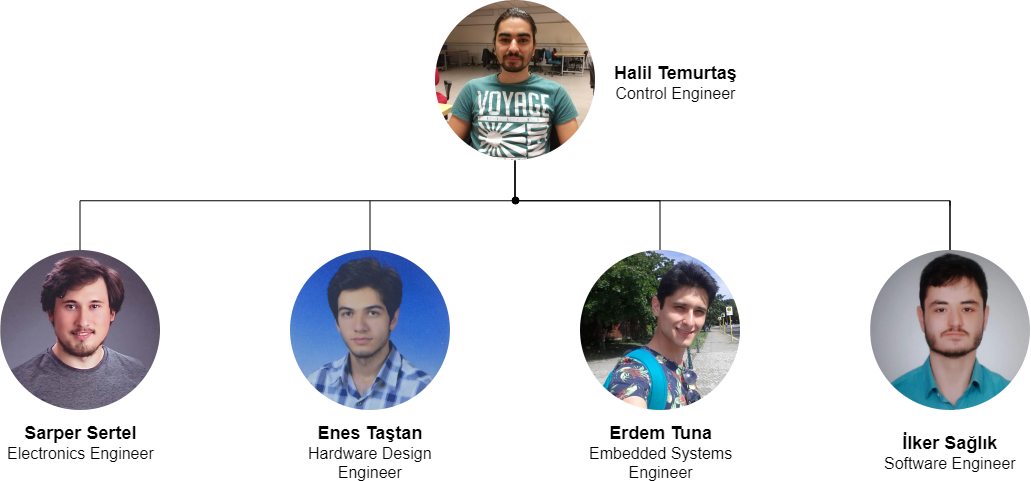
\includegraphics[width=\textwidth,height=\textheight,keepaspectratio]{../../Documents/company/company-tree} 
	\caption{\label{fig:company_tree}Company Tree of DUAYENLER.}
\end{figure}


\section{Requirement Analysis}
	
	\subsection{Pairwise Comparisons for Project Selection}
		Pairwise comparisons technique can be use to assess objectives of the project. Then, these objectives can be very useful as the desired project is selected out of all potential project. For this purpose, tables at \textit{Figures~\ref{fig:pairwise_comp},\ref{fig:project_eval}} is created by consensus of all project-pairs. The weighted objectives are then used to construct the weighted objective tree at \textit{Figure~\ref{fig:objective_tree}}. 

	\begin{figure}[H]
		\centering
		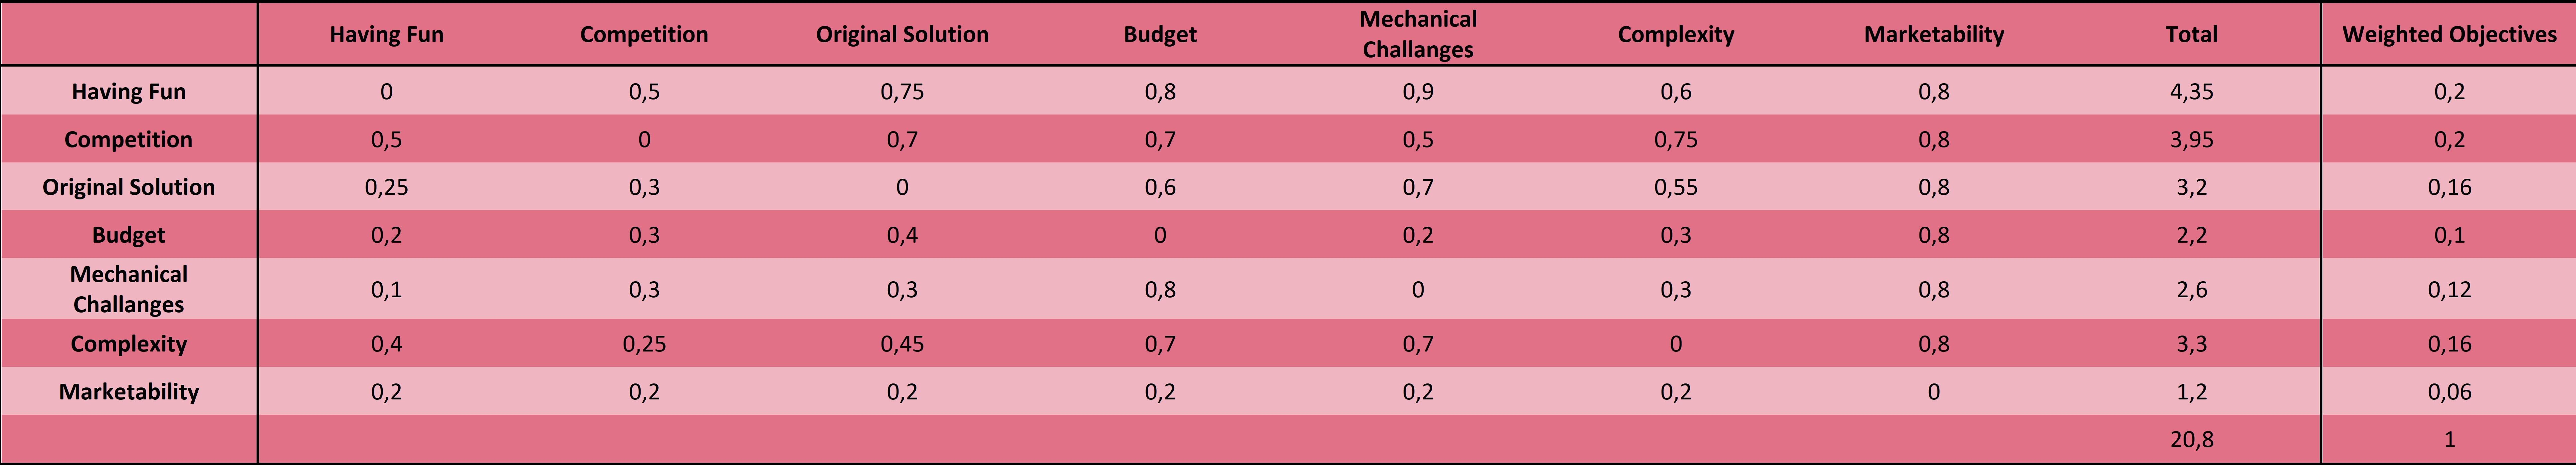
\includegraphics[width=\textwidth,height=\textheight,keepaspectratio]{images/objective_tree} 
		\caption{\label{fig:pairwise_comp}Pairwise Comparison Charts}
	\end{figure}
	
	\begin{figure}[H]
		\centering
		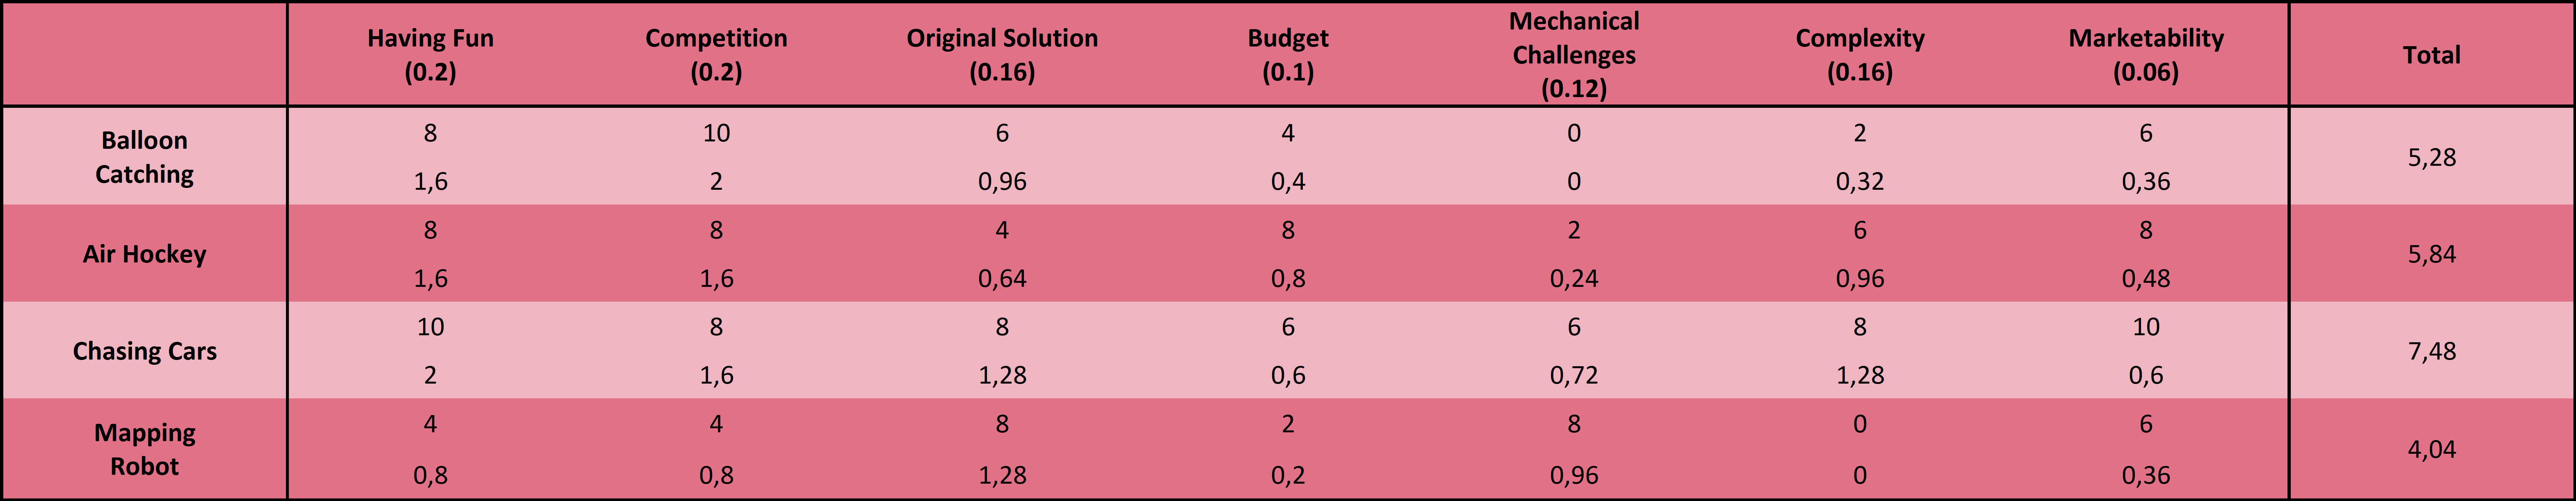
\includegraphics[width=\textwidth,height=\textheight,keepaspectratio]{images/project_evaluation2} 
		\caption{\label{fig:project_eval}Project Evaluation Chart}
	\end{figure}
	
	
	\begin{figure}[H]
		\centering
		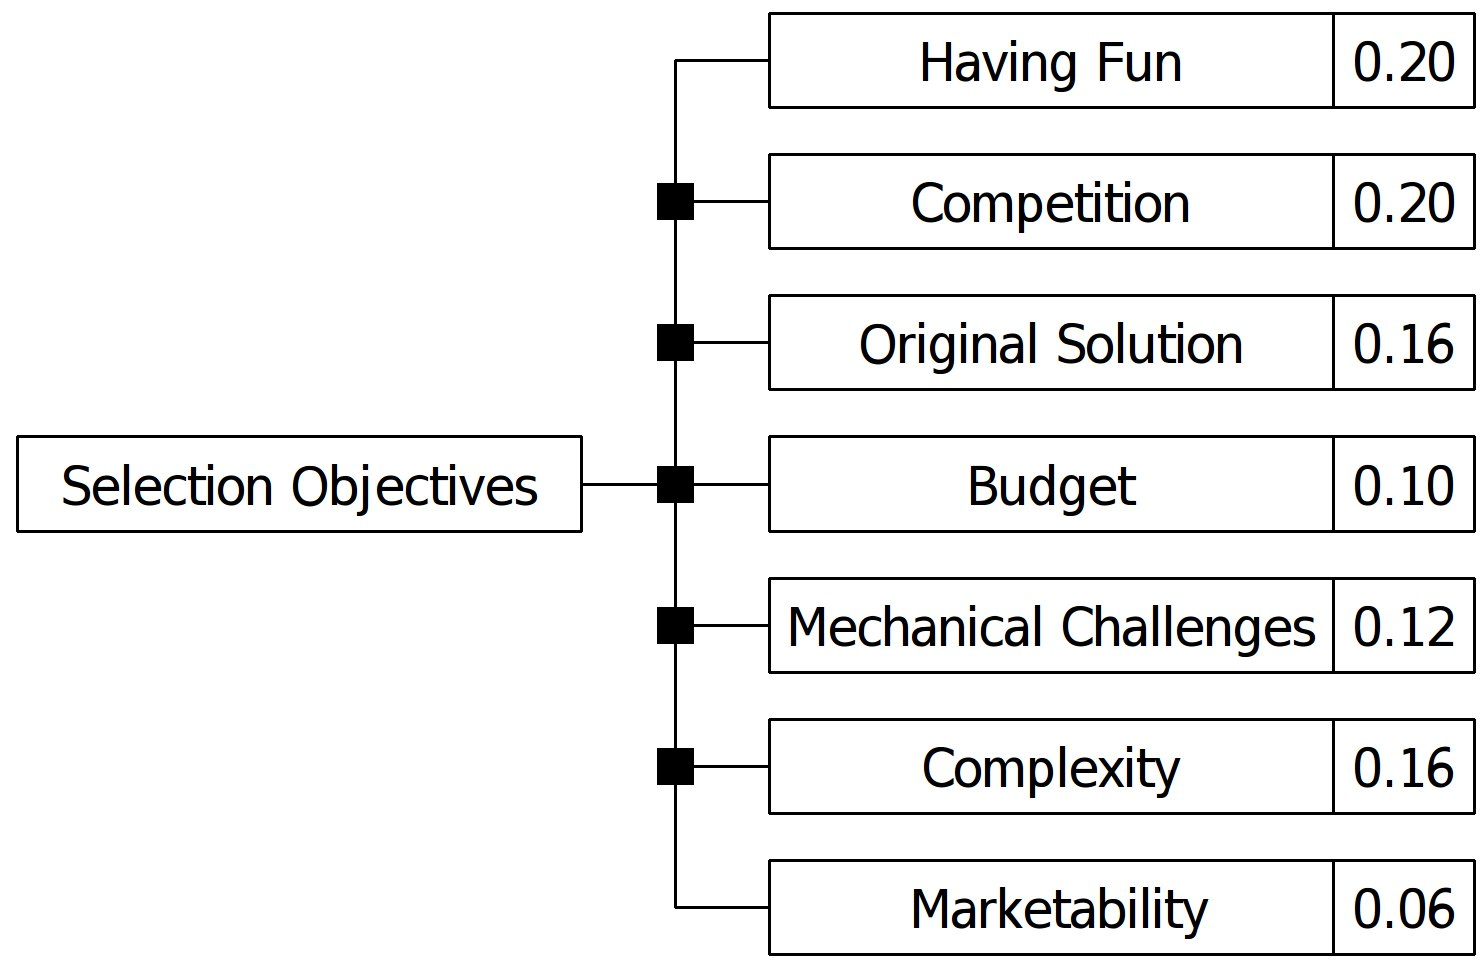
\includegraphics[width=\textwidth,height=\textheight,keepaspectratio]{pre-objective-tree/pre-objective-tree} 
		\caption{\label{fig:objective_tree}Weighted Objective Tree}
	\end{figure}

	
	
	\subsection{Systems \& Subsystems of Chosen Project}	
	
	\begin{figure}[H]
		\centering
		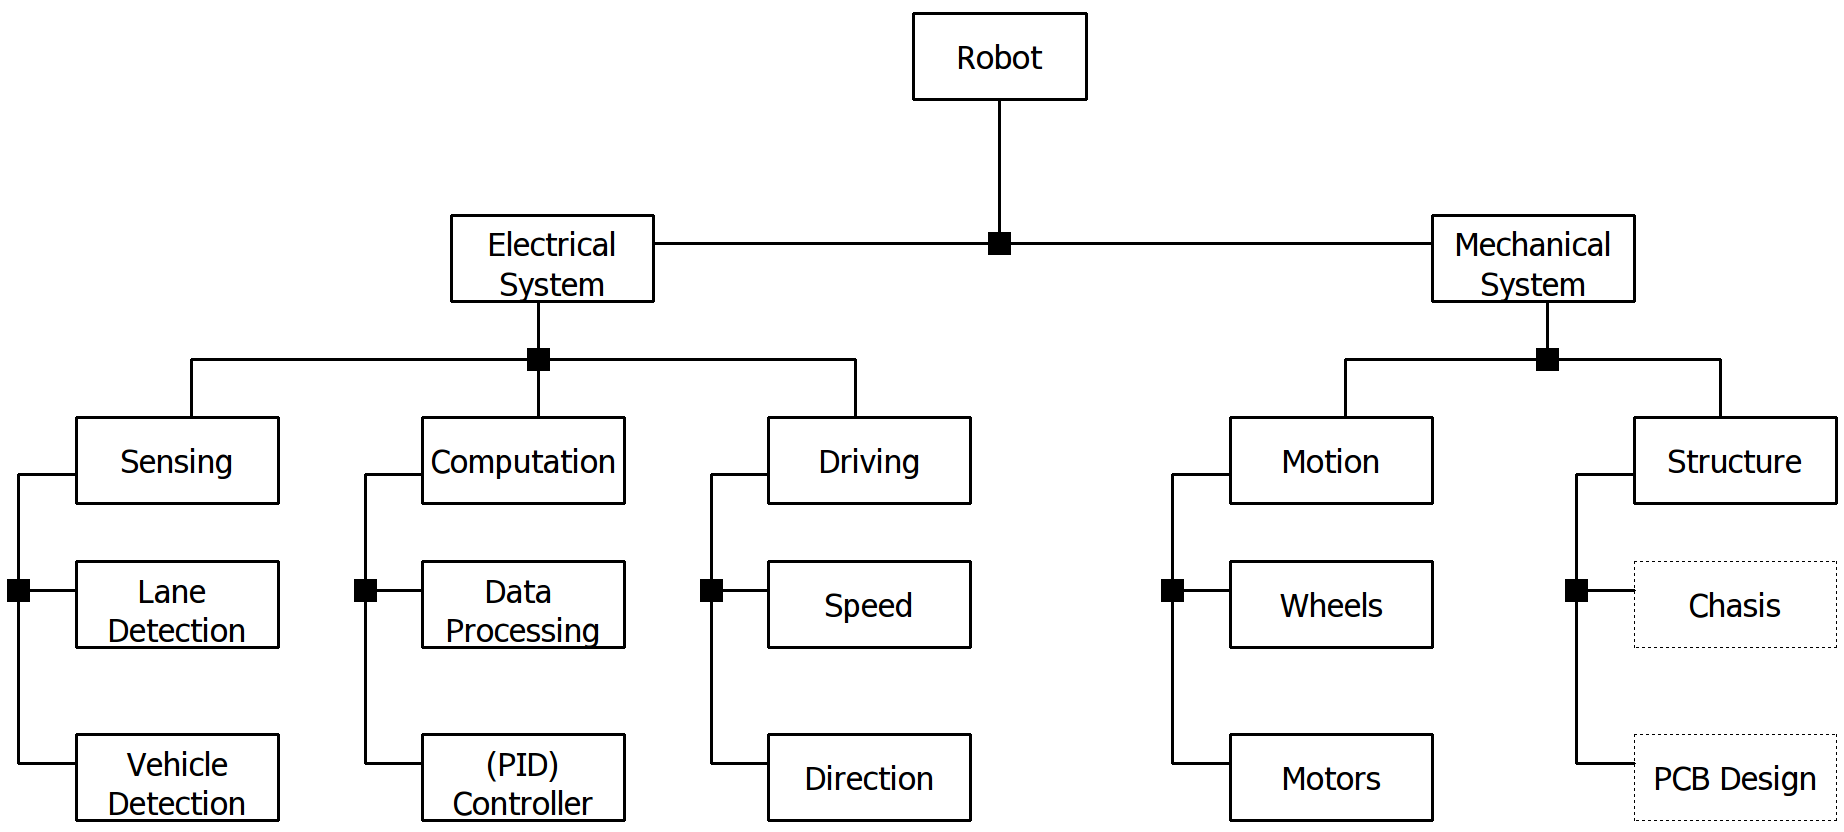
\includegraphics[width=\textwidth,height=\textheight,keepaspectratio]{product-tree/product-tree} 
		\caption{\label{fig:product_tree}Weighted Objective Tree}
	\end{figure}

	\subsection{Solution Alternatives for Systems \& Subsystems }
	
	\subsection{Design Option 1}
	
	\subsection{Design Option 2}
	
	\subsection{Design Option 3}
	
	
	\subsection{Pairwise Comparisons for Solution Selection}	
	
	\begin{figure}[H]
		\centering
		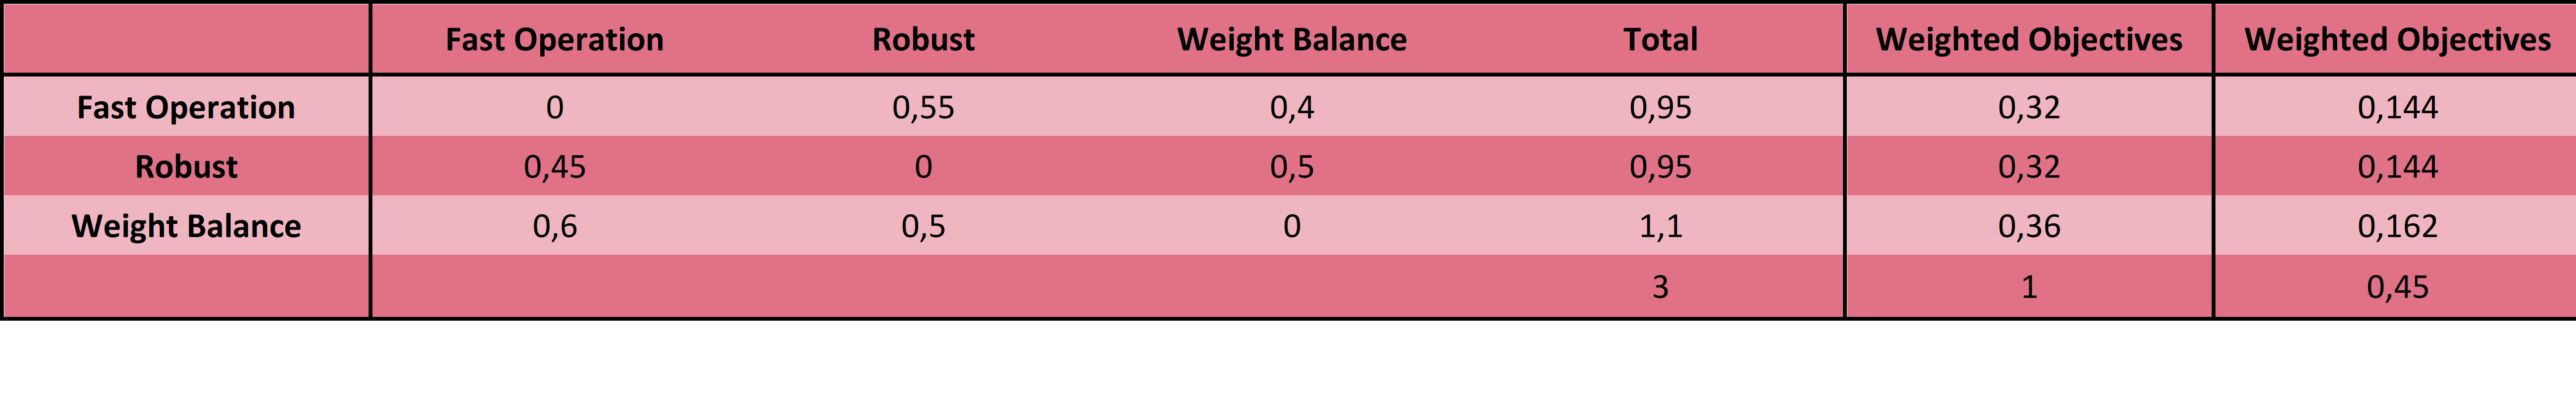
\includegraphics[width=\textwidth,height=\textheight,keepaspectratio]{images/proje_objective_tree_2} 
		\caption{\label{fig:sub_project_objective_tree}Pairwise Comparison Charts for Sub-Objectives}
	\end{figure}	
	
	\begin{figure}[H]
		\centering
		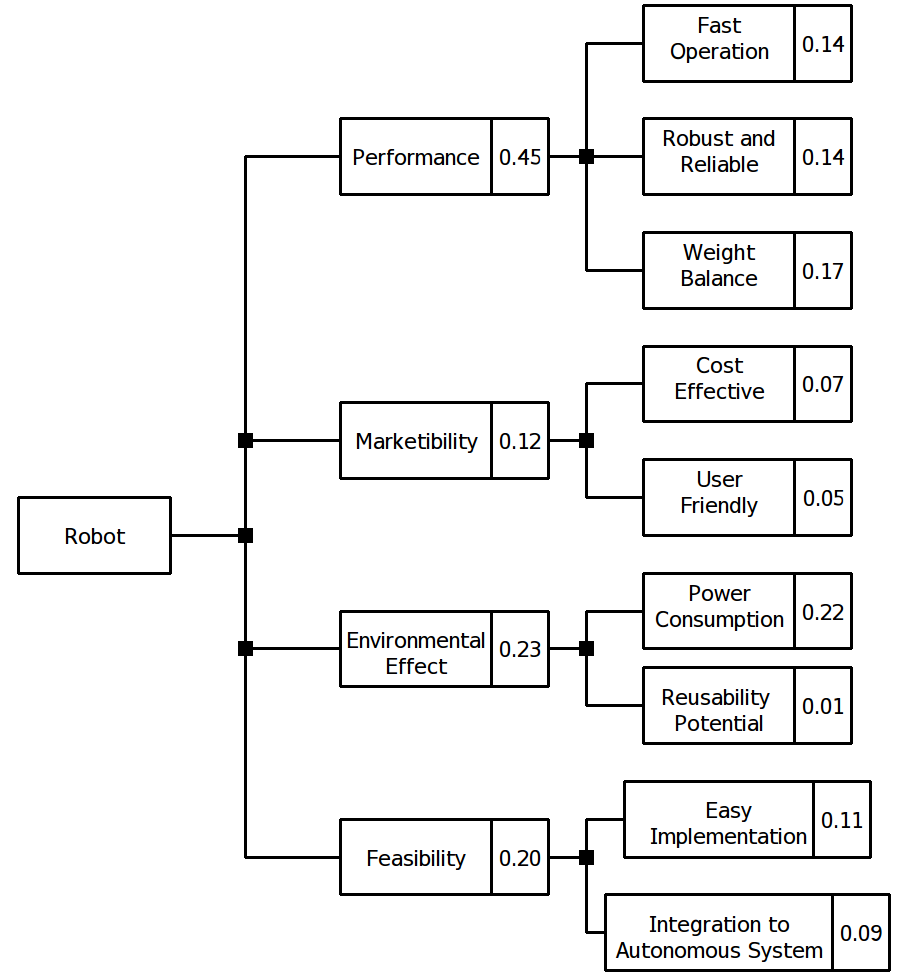
\includegraphics[width=\textwidth,height=\textheight,keepaspectratio]{objective-tree/objective-tree} 
		\caption{\label{fig:product_tree}Weighted Objective Tree}
	\end{figure}
	
	\begin{figure}[H]
		\centering
		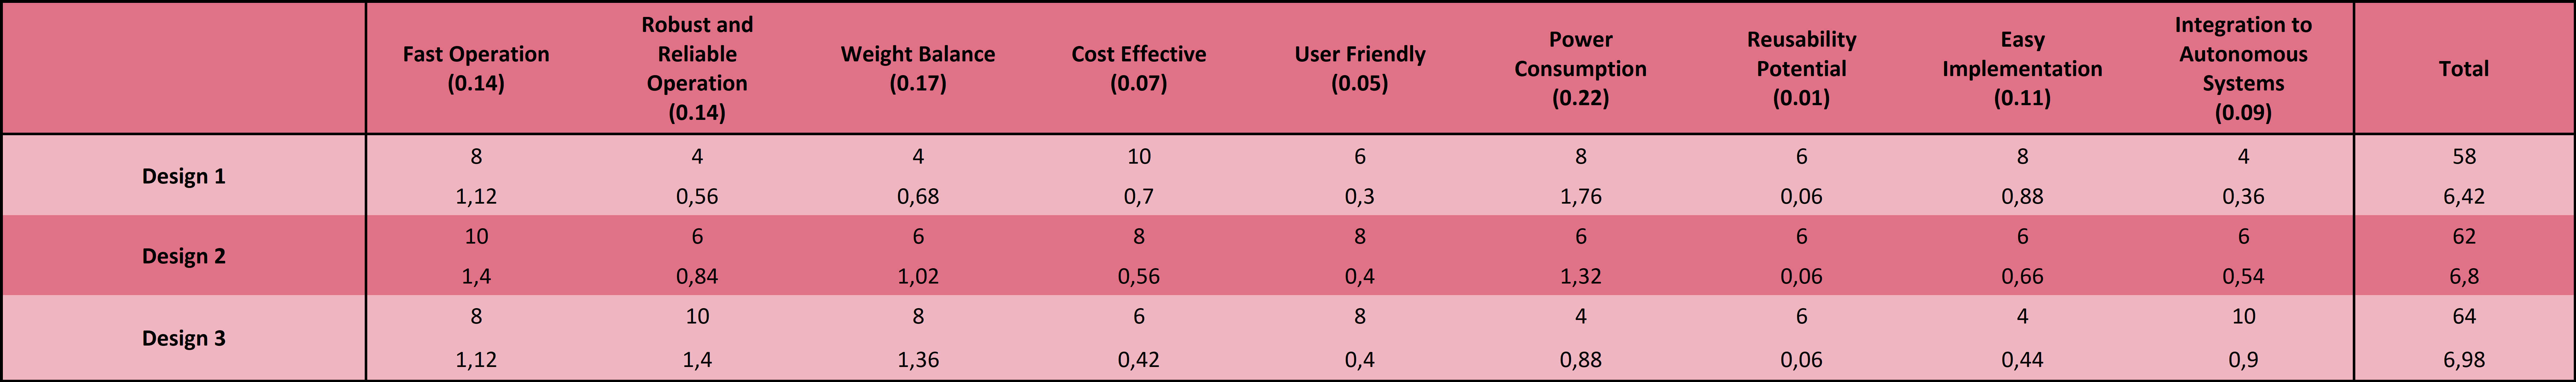
\includegraphics[width=\textwidth,height=\textheight,keepaspectratio]{images/soln_selection} 
		\caption{\label{fig:soln_selection}Pairwise Comparison Charts for Solution Selection}
	\end{figure}


%	\begin{figure}[H]
%		\centering
%		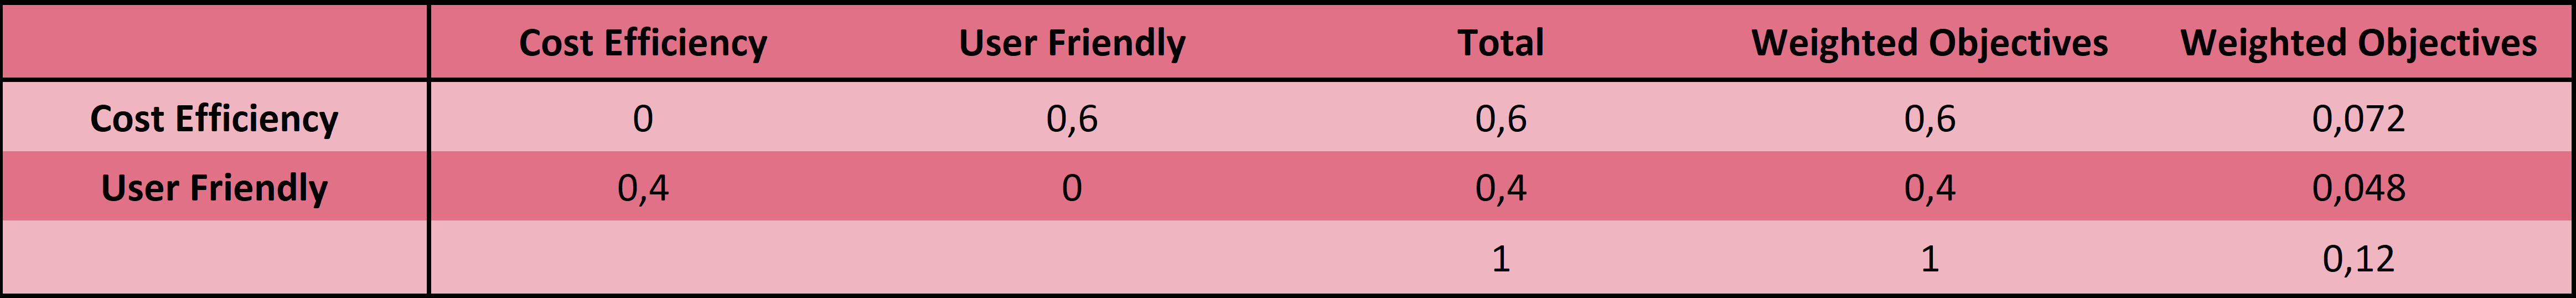
\includegraphics[width=\textwidth,height=\textheight,keepaspectratio]{images/proje_objective_tree_3} 
%		\caption{\label{fig:schedule}Weekly Schedule}
%	\end{figure}


%	\begin{figure}[H]
%		\centering
%		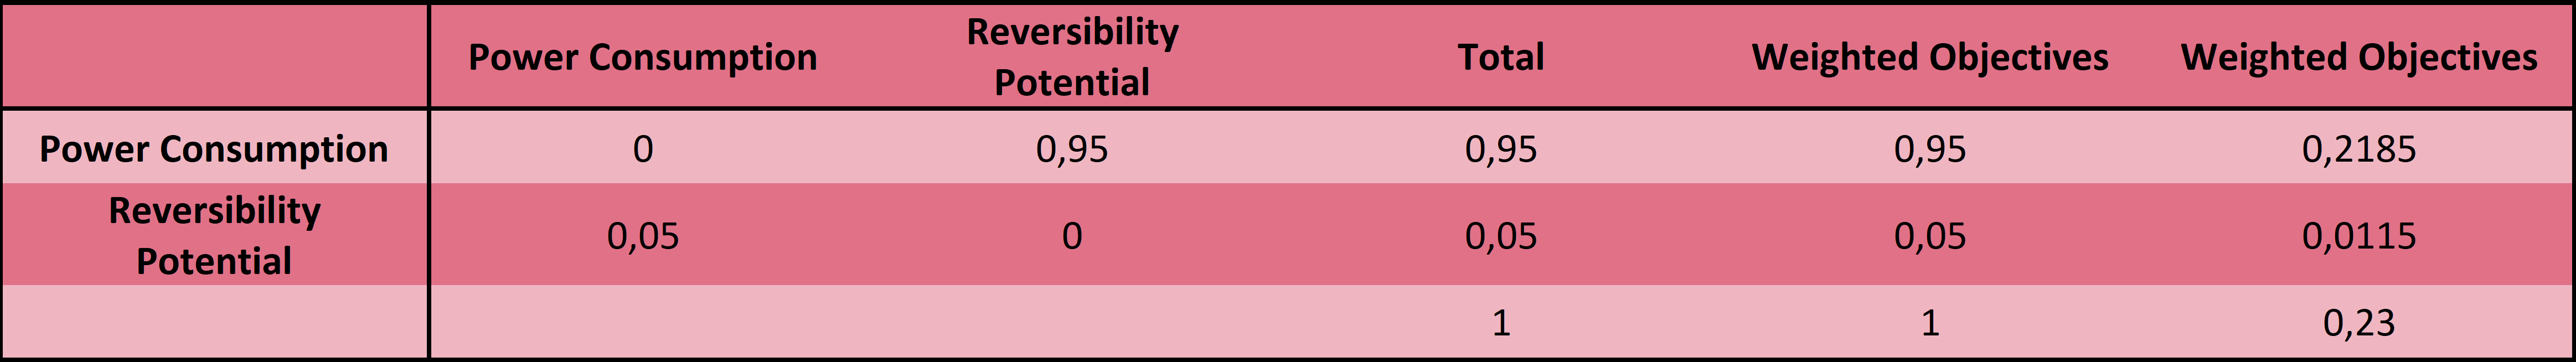
\includegraphics[width=\textwidth,height=\textheight,keepaspectratio]{images/proje_objective_tree_4} 
%		\caption{\label{fig:schedule}Weekly Schedule}
%	\end{figure}

	

\section{Standards Section}


\section{Solution Procedure}


\section{Expected Deliverables}


\section{Conclusion}

\newpage
\begin{appendices}
	
		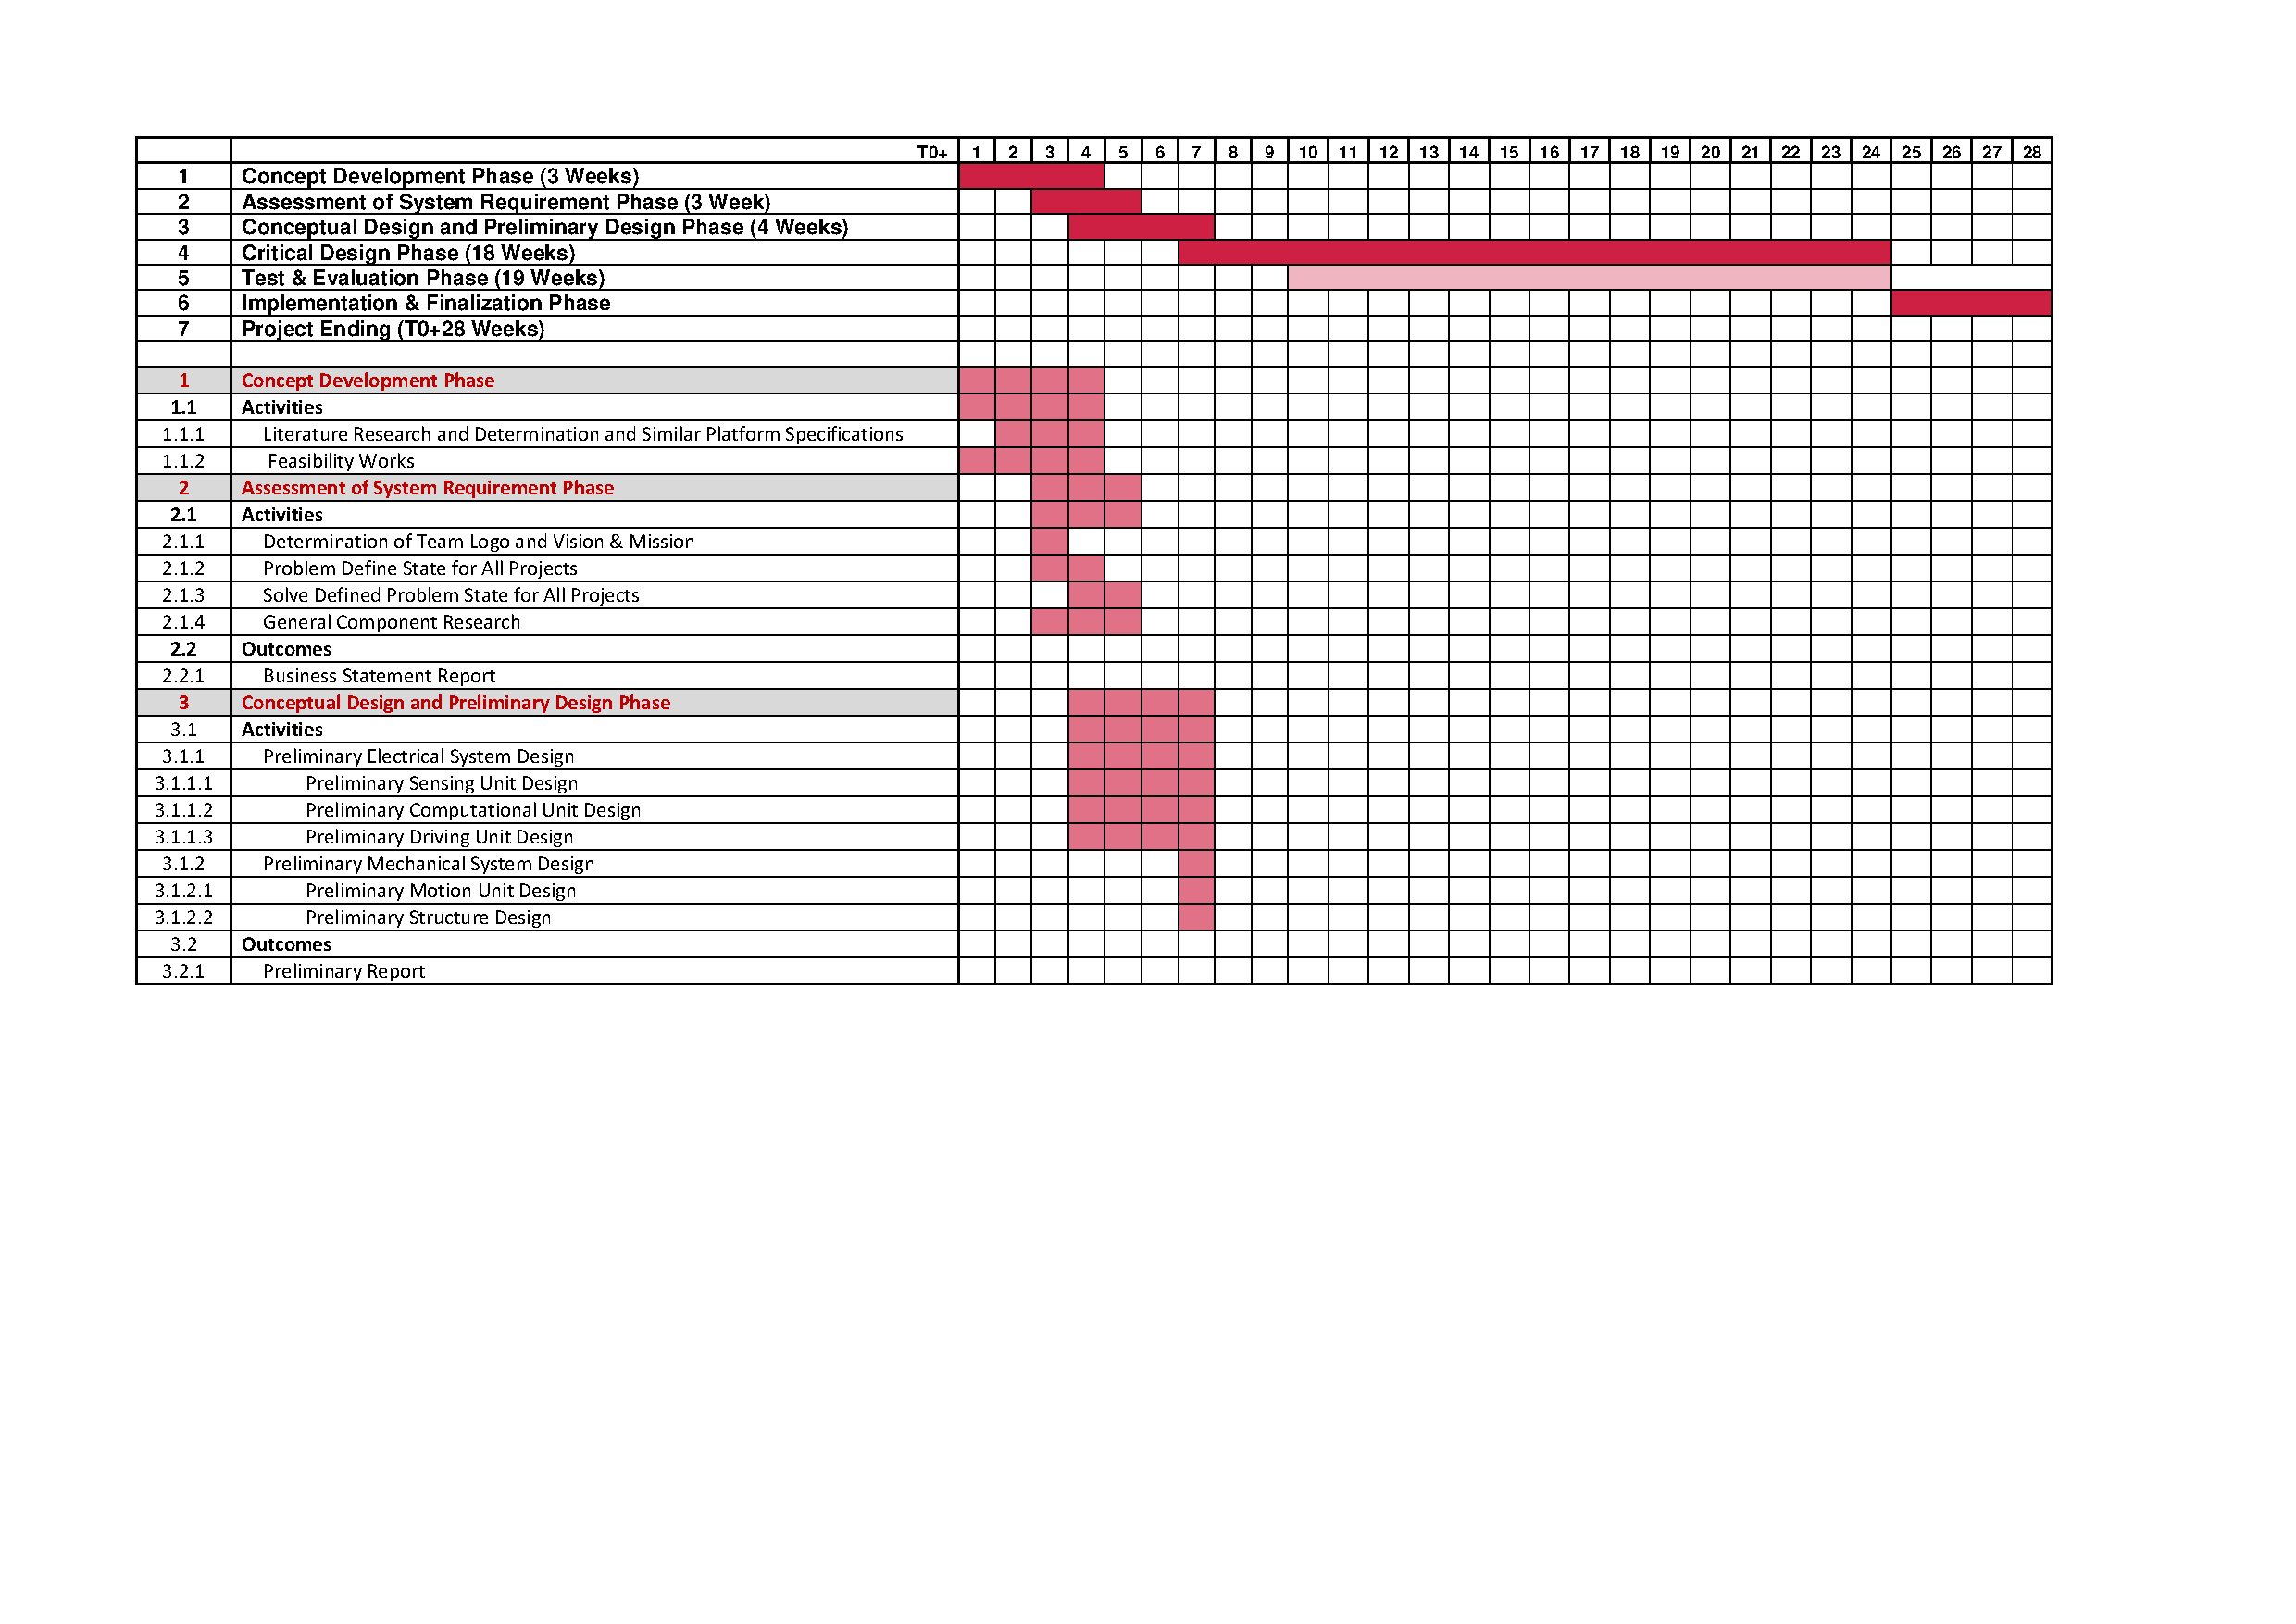
\includepdf[landscape=true,pages=1, scale=0.85,pagecommand=\section{Gannt Chart}]{gannt_chart.pdf}
		\includepdf[landscape=true,pages=2, scale=0.85,pagecommand=]{gannt_chart.pdf}

	
\end{appendices}




\end{document}

%----samples------
%\begin{itemize}
%\item Item
%\item Item
%\end{itemize}

%\begin{figure}[H]
%\center
%\setlength{\unitlength}{\textwidth} 
%
\includegraphics[width=0.7\unitlength]{images/logo1}
%\caption{\label{fig:logo}Logo }
%\end{figure}

%\begin{figure}[H]
%	\setlength{\unitlength}{\textwidth} 
%	\centering
%	\begin{subfigure}{.5\textwidth}
%  		\centering
%  		
\includegraphics[width=0.48\unitlength]{images/logo1}
%  		\caption{\label{fig:logo1}Logo1 }
%	\end{subfigure}%
%	\begin{subfigure}{.5\textwidth}
%  		\centering
%		
\includegraphics[width=0.48\unitlength]{images/logo2}
%  		\caption{\label{fig:logo2}Logo2}
%	\end{subfigure}
%\caption{\label{fig:calisandegree} Small Logos   }
%\end{figure}
	
%\begin{table}[H]
%  \centering
% 
%    \begin{tabular}{c|c|c}
%       $$A$$ & $$B$$ & $$C$$ \\ \hline
%       1 & 2 & 3  \\ \hline
%       2 & 3 & 4  \\ \hline
%       3 & 4 & 5  \\ \hline
%       4 & 5 & 6  
%      
%  \end{tabular}
%  \caption{table}
%  \label{tab:table}
%\end{table}
	
%\begin{table}[H]
%  \centering
% 
%    \begin{tabular}{c|c|c}
%       \backslashbox{$A$}{$a$} & $$\specialcell{ Average deviation \\ after subtracting out the  \\ frequency error }$$ & $$C$$ \\ \hline
%       \multirow{2}{*}{1} & 2 & 3  \\ \cline{2-3}
%        & 3 & 4  \\ \hline
%       3 & \multicolumn{2}{c}{4}  \\ \hline
%       4 & 5 & 6  
%      
%  \end{tabular}
%  \caption{table}
%  \label{tab:table}
%\end{table}
%-----end of samples-----